\section{Introduction}
\subsection{Motivation}
With the rise of simulation and big data analytics as new foundations of all modern science,
access to large scale \ac{HPC} systems has become paramount for good research. Furthermore,
as the area of machine and deep learning progresses, with models containing over one billion
parameters \cite{gpt4param},  local computation becomes everless feasable, resulting in the 
rise of \ac{HPC} usage amongst various domains.\\

This report is written as an addition to my student research at the \ac{GWDG}. The \ac{GWDG} is the
data center of the University of Göttingen and the data and IT competence center of the 
Max Planck Society with its own \ac{HPC} department, running four large scale \ac{HPC} systems:
The \ac{SCC}, Emmy, Grete, and CARO:
\begin{itemize}
\item \textbf{\ac{SCC}}\cite{SCC}: The \ac{SCC} is the oldest cluster maintained 
by the \ac{GWDG}. Its user group is comprised of all researchers of the Max Planck Society as 
well as all (student) researchers of the University of Göttingen. It is a very heterogenous system,
based on several different CPUs and GPUs generations, located over several locations within 
Göttingen. In total, it has 18,376 CPU Cores, 99 TB RAM and 5.2 PiB of Storage.
\item \textbf{Emmy}\cite{Emmy}: Together with the Lise\footnote{
\url{https://www.zib.de/research_services/supercomputing}} cluster provided by the ZIB, Emmy is 
part of  the fourth supercomputer generation of the HLRN\footnote{Norddeutscher Verbund für Hoch- 
und Höchstleistungsrechnen \url{https://www.hlrn.de/}}. It can be used by all HLRN and NHR users.
Ranking 133th at the TOP500\footnote{As of November 2023.}, Emmy is the biggest cluster hosted by
the \ac{GWDG}. It consists of 111,464 CPU Cores distributed over 1423 compute nodes resulting 
in a total peak compute power of 5.95 PetaFLOP/s.
\item \textbf{Grete}: Grete is a GPU \ac{HPC} cluster, formally part of the NHR system.
It features 158 nodes with 2 AMD Epyc 7513 CPUs and four NVIDIA A100 GPUs each, connected through fast
Infiniband fabric. As of November 2023, Grete is rank 142 of the TOP500.
\item \textbf{CARO}\cite{CARO}: Analagously to Emmy provided for the NHR, CARO is a compute cluster
hosted for the DLR\footnote{Deutsches Zentrum für Luft- und Raumfahrt \url{https://www.dlr.de/en}}.
With its 1364 compute nodes with 175,744 CPU Cores and 3.46 PetaFLOP/s it ranks 228th on TOP500.
\end{itemize}

As the sheer number of nodes makes individually inspecting each one impossible, a centralized
monitoring solution is required. Beyond getting an basic understanding on which node is alive, 
monitoring systems serve several important purposes. With an aggregated view, system admins can
understand the usage pattern of users. Furthermore, it can be used as a means of load balancing 
for detecting preventable bottlenecks such as suboptimal job queue usage. Additionally, monitoring
allows for better demand analysis and forecasting, allowing for more efficient, just in time 
hardware upgrades.

\subsection{Goals and Contributions}

As the time of this writing, the GWDG has two different, Grafana-based monitoring solutions for 
the \ac{SCC} and Emmy/Grete. The goal of this report is to evaluate the performance viability of
unifying both monitoring solutions, replacing \ac{SCC}'s InfluxDB\footnote{
\url{https://www.influxdata.com/products/influxdb-overview/}} and Telegraf\footnote{
\url{https://www.influxdata.com/time-series-platform/telegraf/}} with Prometheus and 
\texttt{node\_exporter}.
As part of this, the following contributions were made:
\begin{itemize}
\item Designing a methodology for benchmarking a pull-based monitoring system.
\item Designing a methodology for benchmarking a pull-based monitoring client daemon, both in 
terms of throughput and the performance degradation caused to typical, throughput-oriented 
\ac{HPC} load.
\item Benchmarking the performance and scalability of Prometheus for a \ac{HPC} use case.
\item Benchmarking the performance and performance penalty of \texttt{node\_exporter} for a 
\ac{HPC} use case.
\end{itemize}

\subsubsection{Structure}
Starting with Section 2, the general topics of monitoring, time series databases and
Prometheus get introduced. Related work about time series database performance will be analyzed.
After that, in Section 3, the benchmark methodology for both Prometheus itself as well as
\texttt{node\_exporter} will be explained. Then, in Section 4, the results of those benchmarks
will be shown. After a short discussion in Section 5, the work will be concluded in Section 6.

\section{Background: Monitoring}
Monitoring consists of 2 important components. On the one hand, it is the continuous 
collection of mostly numerical data and metrics from various systems. On the other hand, it 
is the aggregation and analysis of this collected data/metrics within a certain period of 
time, up to real-time monitoring.

Several different kinds of metrics can be analyzed using monitoring systems. From typical
system metrics such as CPU, RAM, disk, or network usage to monitoring whole server racks
with power and cooling statistics as well as application specific metrics such as databases
or webservers.

Most monitoring systems follow the collector/database/dashboard architecture. On each node,
a \emph{collector} is running as a daemon, exposing the internal metrics for an centralized
database, aggregating all nodes. Those databases are usually either general, document-based
NoSQL databases such as MongoDB\footnote{\url{https://www.mongodb.com/}} and 
Elasticsearch\footnote{\url{https://www.elastic.co/elasticsearch}} or specialized \acp{TSDB}
such as InfluxDB\footnote{\url{https://www.influxdata.com/}} or Prometheus\footnote{
\url{https://prometheus.io/}}.

To provide an taxonomy, most monitoring systems can be categorized on two dimensions:

\paragraph{Cloud-based or On-Premise:} Monitoring systems can either be managed, cloud-based 
or self-hosted, on-premise services. Both have their advantages and disadvantages.

Cloud-based monitoring services such as Datadog\footnote{\url{https://www.datadoghq.com/}}
or Splunk\footnote{\url{https://www.splunk.com/}} have several advantages. By using an 
externally hosted service, it simplifies the overall monitoring maintenance. By not requiring
hardware for another service, it lowers the barrier of entry. Furthermore, since the whole
monitoring stack is written by the same manufacturer, it allows for tighter integration.

On-Premise hostings, on the other hand, also have several advantages over the cloud-based 
solutions. Since they are part of the local network, they are easier to integrate into current
infrastructure, even those parts that one doesn't want to publically expose such as Active 
Directory. Additionally, it mitigates potential security and privacy risks, especially for data
that could either pose a security risk such as showing applicable vulnerabilities or data that is
legally not allowed to be processed off-premise such as sentitive user data. Lastly, while the 
software stack is more heterogenous, it allows for more specialization based on the users needs.

\paragraph{Push or Pull:} There are two different paragigms in data gathering:

In the more common \emph{push} paradigm, the data-collecting daemon sends the data to an API 
endpoint. This has multiple advantages: First, it is easier for firewalls, because it does not
need any inbound connection establishment. It is also less overhead for the \ac{TSDB} since it
just needs to passively recieve the data. Lastly, it is easier to send non-aggregated raw data,
since the client can decide when it has enough data to send to the database.

In the \emph{pull} paradigm, the \ac{TSDB} itself iterates over, and fetches all metrics, which
are exposed as newline-seperated key-value pairs through an specified HTTP-endpoint. The biggest
advantage is that the \ac{TSDB} can't be overwhelmed with requests since it implicitly rate-limits
itself through the amounts of outgoing requests. Furthermore, it allows for lazy and just-in-time 
fetching of data, reducing the overall overhead in the network.

The \ac{GWDG} uses both push and pull \acp{TSDB} in the \ac{SCC} and Emmy cluster respectively. 

\subsection{Current Architecture: GWDG SCC}

The \ac{SCC} uses an push-based architecture: On every node, the plugin-powered Telegraf 
daemon collects all metrics, which are then send to the InfluxDB \ac{TSDB}. Finally, this database
gets queried using the legacy InfluxQL by Grafana\footnote{\url{https://grafana.com/}} as 
configured in the dashboards.

\begin{figure}[H]
  \centering
  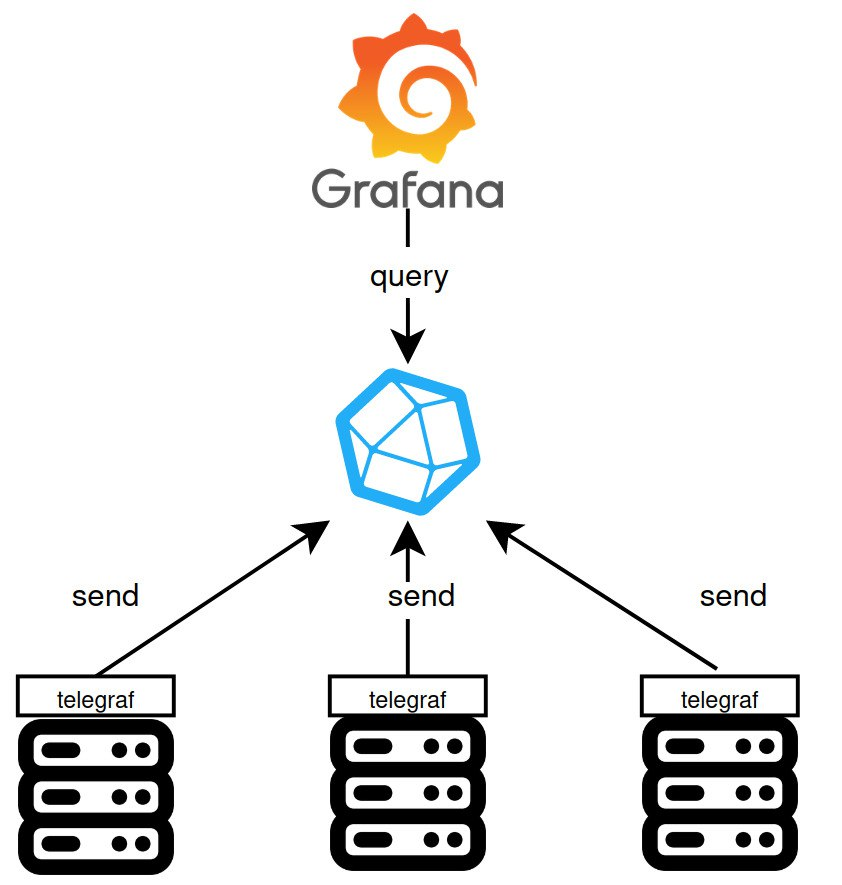
\includegraphics[width=0.5\textwidth]{./assets/influx.jpeg}
  \caption{The InfluxDB-based push-setup for the SCC.}
\end{figure}


\subsection{Current Architrecture: HLRN Emmy}
For Emmy, a pull-based architecture is used. The node\_exporter\footnote{
\url{https://github.com/prometheus/node_exporter}} exposes the \texttt{/metrics} endpoint, to which
the Prometheus database connects to when fetching the data. The aggregated data also gets queried
through pre-made Grafana dashboards with PromQL.

\begin{figure}[H]
  \centering
  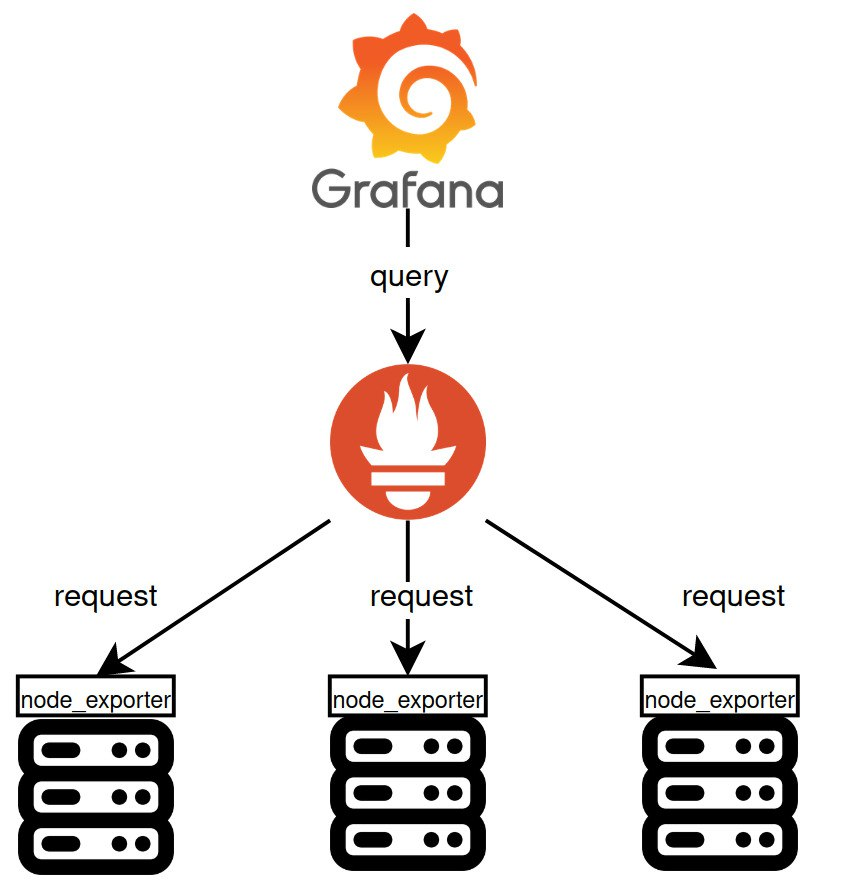
\includegraphics[width=0.5\textwidth]{./assets/prometheus.jpeg}
  \caption{The Prometheus-based pull-setup for Emmy.}
\end{figure}

\subsection{Prometheus}
More than just a \ac{TSDB}, Prometheus is a pull-based systems monitoring toolkit. Originally 
developed at SoundCloud, it is now a non-commercial open source project hosted by the \ac{CNCF},
which is a part of the Linux Foundation. It expoeses the pull metrics via \texttt{node\_exporter},
which then get scraped by the Prometheus server into its \ac{TSDB}, which can then be queried through
PromQL, its own query language.

\begin{figure}[H]
  \centering
  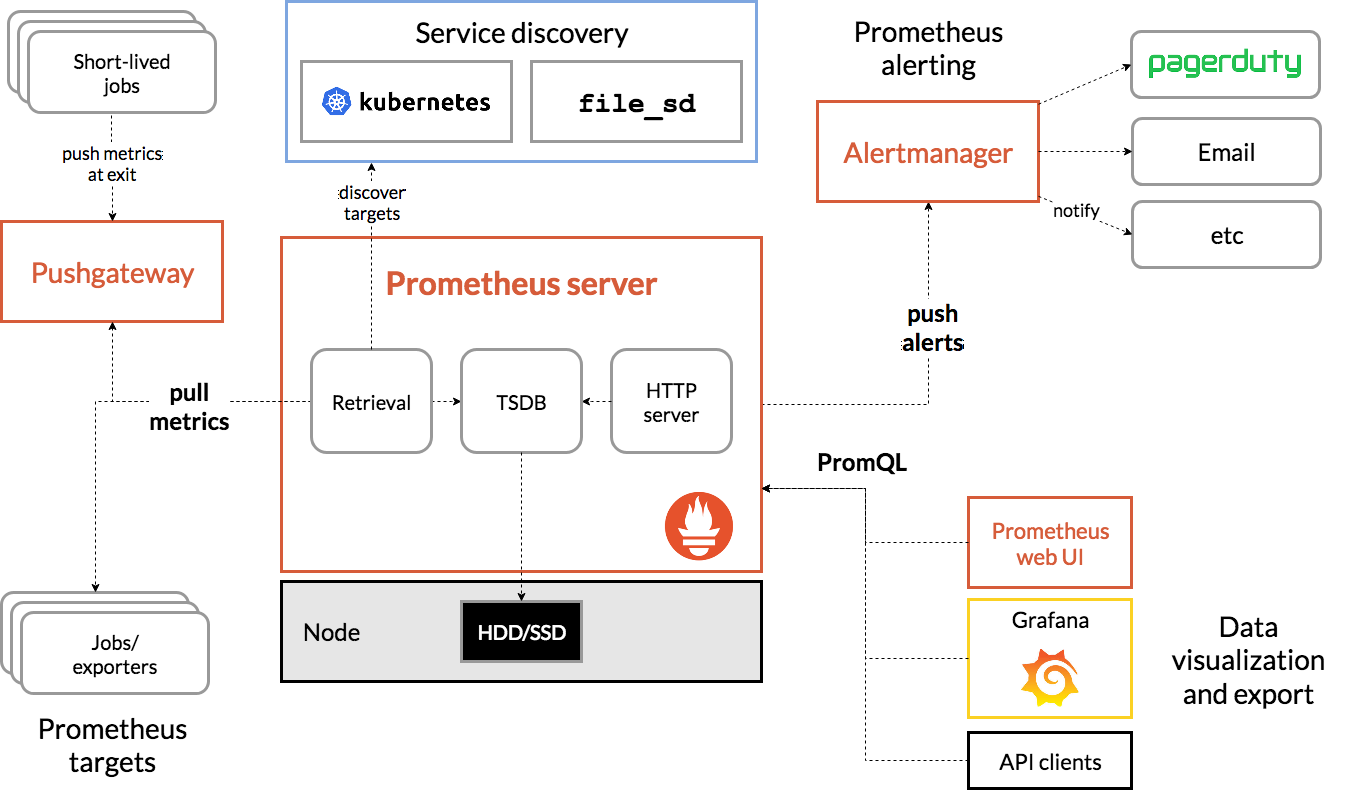
\includegraphics[width=\textwidth]{./assets/promarch.png}
  \caption{Prometheus high level architecture \cite{promarch}.}
\end{figure}

\subsection{TSDB Performance Evaluation}
While there are several papers on \ac{TSDB} performance evaluation, most benchmarking was mainly
done by different vendors. In this section, we will cover one formal publication as well as two
industry standards for push and pull based database benchmarking.

The most actively maintained academic benchmark was first published by Liu and Yuan in 2019 \cite{benchmark_paper}.
It is maintained to this day. While it surrently only supports Push-based metrics, it supports not
only traditional \ac{TSDB} such as InfluxDB or TimeScaleDB but also classical SQL-based databases
such as SQLite or Microsoft SQL Server. It also supports several benchmarking scenarios testing
both write and query performance.

But the canonical benchmarking suite for push-based \acp{TSDB} is the \ac{TSBS} \cite{tsbs}, 
maintained by Timescale, the maintainer of timescaledb\footnote{\url{https://www.timescale.com/}}, a 
time-series database packaged as an PostgresSQL. Initially developed by an external contractor
for InfluxData as \texttt{influxdb-comparisons} \cite{influxcomp}, it supports most \acp{TSDB}.
It is split into 3 different, purely distinct phases: Data and query generation, data insertion,
and query execution. This is done to minimize the load generator overhead for more reliable results.

Due to the constant load configured on the server side instead of the load generator side, pull-based
\ac{TSDB} benchmarking is more difficult. Although still pretty new, the only well maintained
benchmark suite for prometheus-like systems is \texttt{prometheus-benchmark} \cite{prombench}, developed by 
VictoriaMetrics\footnote{\url{https://victoriametrics.com/}}, a competitor to Prometheus. It supports
VictoriaMetrics as well as Prometheus based Grafana's Mimir\footnote{\url{https://grafana.com/oss/mimir/}}
and the \ac{CNCF}-maintained Prometheus clustering solutions Cortex\footnote{\url{https://github.com/cortexproject/cortex}}
and Thanos\footnote{\url{https://github.com/thanos-io/thanos/}}. Unfortunately, it can not be used for
this benchmark as it expects a Kubernetes-based cloud environment while this use case is around \ac{HPC} usage.

Unfortunately, due to the competitive nature of the highly funded No-SQL startup space, both
benchmarks suits are susceptible to commercial incentives.


\section{Benchmark Methodology}
This section will cover the design and methodology behind all benchmarks. In particular, the following
benchmarks were designed as part of this report:

\begin{itemize}
  \item Measuring the isolated performance of the metric gathering function within the \texttt{node\_exporter} daemon.
  \item Measuring the end-to-end performance of the \texttt{node\_exporter} daemon with different HTTP load generators.
  \item Measuring the scalability of Prometheus by increasing the number of daemons to fetch from.
  \item Measuring the performance penalty of \texttt{node\_exporter} on an running \ac{HPC} job.
\end{itemize}

Note that the code for all benchmarks \cite{my_repo} as well as the patched \texttt{node\_exporter} \cite{my_node_exporter}
can be found on Github.

\subsection{Setup}

For the \texttt{node\_exporter} performance benchmarks as well as the Prometheus benchmark, an \ac{HPC} 
gcn2 type node from the HLRN Emmy cluster was used. This node has two Xeon Platinum 9242 with 48 cores each
as well as 376GB of RAM. The servers were solely used for the benchmarks, thus resulting in
no noisy neighbour problems.

In order to facilitate a more minimal operating system with less running services, the jitter-based 
performance penalty benchmark was done locally on a Dell Latitude 7420 running a minimal
Debian bookworm on an USB stick. The Dell has a quad-core Intel i5-1145G7 as well as 16GB of RAM.

The \texttt{node\_exporter} benchmarks uses a precompiled node exporter of version 1.7.0\footnote{With the following collectors enabled: cpu, cpufreq, infiniband, meminfo, netdev, vmstat.}
For the isolated metric gathering benchmark, 
\texttt{node\_exporter} was forked from version 1.7.0. For Prometheus, a Ubuntu 22.04 based singularity
container was used as a basis, containing a Prometheus version 2.45.1. The Dockerfile is also available
in the repository \cite{my_repo}.

\subsection{\texttt{node\_exporter}}
\subsubsection{Metric Gathering}

When requesting all metrics via the \texttt{/metrics} HTTP endpoint, \texttt{node\_exporter} runs the following
function:

\begin{listing}[H]
  \inputminted{go}{./gather.go}
  \caption{How the metrics are collected in \texttt{collector/collector.go}}
\end{listing}

So when requesting the metrics, \texttt{node\_exporter} spawns a new green thread for each metric plugin, 
awaiting all results in a fork-join like model with a semaphore. Instead of benchmarking the single function
by mocking a realistic application state, the Collect function was patched as follows:

\begin{listing}[H]
  \inputminted{go}{./gather_patched.go}
  \caption{The patched collector measuring the collection time. Note that the \texttt{RealCollect} function contains the same code as the unpatched \texttt{Collect}.}
\end{listing}

Further small patches had to be done to fix any errors, see the reporitory for more information \cite{my_node_exporter}.

\subsubsection{End to End}
The end-to-end benchmarks measured the throughput using traditional HTTP benchmarking. In particular, two different
benchmarking tools were used:
\begin{itemize}
  \item \textbf{wrk} \cite{wrk} is a popular, CLI-based HTTP benchmarking tool written in C. Due to its optimized
    performance it can serve as a baseline optimal throughput. In order to further improve throughput, it keeps
    all connections open.
  \item \textbf{go-wrk} \cite{go-wrk} is a reimplementation of wrk in the Go programming language, using gos
    green threads for the load generation.
\end{itemize}
All benchmarks are measured using \texttt{vmwstat 1}. The benchmarks can be divided into three different kinds.
\begin{enumerate}
  \item \textbf{wrk sequential}: Using a single thread and a single connection, this is the most realistic load,
    as metrics are usually only crawled by a single Prometheus as well. This is also the simplest possible benchmark;
    just send as fast as possible.
  \item \textbf{wrk parallel}: Scaling along the number of connections and threads
\end{enumerate}
% - All benchmarks are measured using `vmstat 1`
% - We have three types of benchmarks
%   - wrk seq
%     - Most realistic load, as one usually has a single prometheus
%     - simplest benchmark: we just blast as fast as possible with 1 thread
%   - wrk par
%     - It keeps the HTTP connections open for maximizing throughput.
%     - While it maximizes throughput, it is not realistic as prom wouldnt do that!
%     - scale along threads and HTTP connections
%   - go-wrk par
%     - it uses the same go `net` lib as prom
%     - It doesnt keep connections open but is highly parallel with go's green threading model
%     - Scale along go-threads
% - For the parallel benchmarks, we start it with some kind of parallelism for some amount
%   then increase parallelism in a step and so on and so fourth:
%   - We also scale along the axis of number of processe consumed by node exporter through the
%     GOMAXPROCS
%     - Note that even with n=1 go threads can still highly improve performance by fixing I/O idle
% - Fully automatic pipeline
\subsubsection{Jitter}
% - Why we think this could be a problem
%   - As mentioned before it spawns up several green threads
%   - Thus more memory footprint, thus potentially wasting the whole CPU cache
% The C file
\subsection{Prometheus}
% - All benchmarks are measured using `vmstat 1`

% - We mocked node exporter
%   - TODO how often it checks; the whole prometheus conf
%   - TODO fastapi 0.104 uvicorn 0.24 single route
%   - TODO only integers, configurable amount of metrics, all nodes have same metrics
%   - TODO how we did randomness with urandom times mersenne warmup
%   - TODO how we count the requests to see whether sth is skipped
%     - Locking global counter
%     - asynccontextmanager
%     - unique filename through pid

% - High level (automatized) workflow.
%   - Give number of mock clients as cli param by providing a port range
%   - Create a dynamic prom cfg for those ports and a 10sec interval to bind-mount in via
%     singularity
%   - spawn all python mock processes in the port range, 1 process per port
%   - Start `vmstat 1`
%   - Start the singularity container with prometheus and the tmp config as well as the 
%     data directory binded in
%     - Explain that the data directory is needed for write ops in footnote
%   - sleep for the amount of the benchmark
%   - terminate prom, then vmstat, then all mock exporter
%     - Terminate == SIGTERM

\section{Results}
\subsection{\texttt{node\_exporter}}
\subsection{Prometheus}

\section{Discussion}
% Node Exporter:
% - we used /dev/urandom, not perlin noise. This is less realistic but less overhead
%   - Even more, the aforementioned tsbs has some predefined data gen
%     - Also they split up the step to avoid the overhead; for us too much IO overhead
%       - Note that we have a convert script to JSON in the repo
% - The mock reporter benchmarks were slower than they had to be
%   because I also piped out all curl results, which added up to 20GB IO :D

\section{Conclusion}
